\section{\diff{Design Details}}

\subsection{Implementation}
\label{sec:impl}

%Question to answer:
%\begin{itemize}
%\item Where is the user input?
%\item Where is admission control?
%\item Where is Scheduler?
%\item How to guarantee the resource?
%\item How resources are allocated?
%\end{itemize}

\begin{figure}
\centering
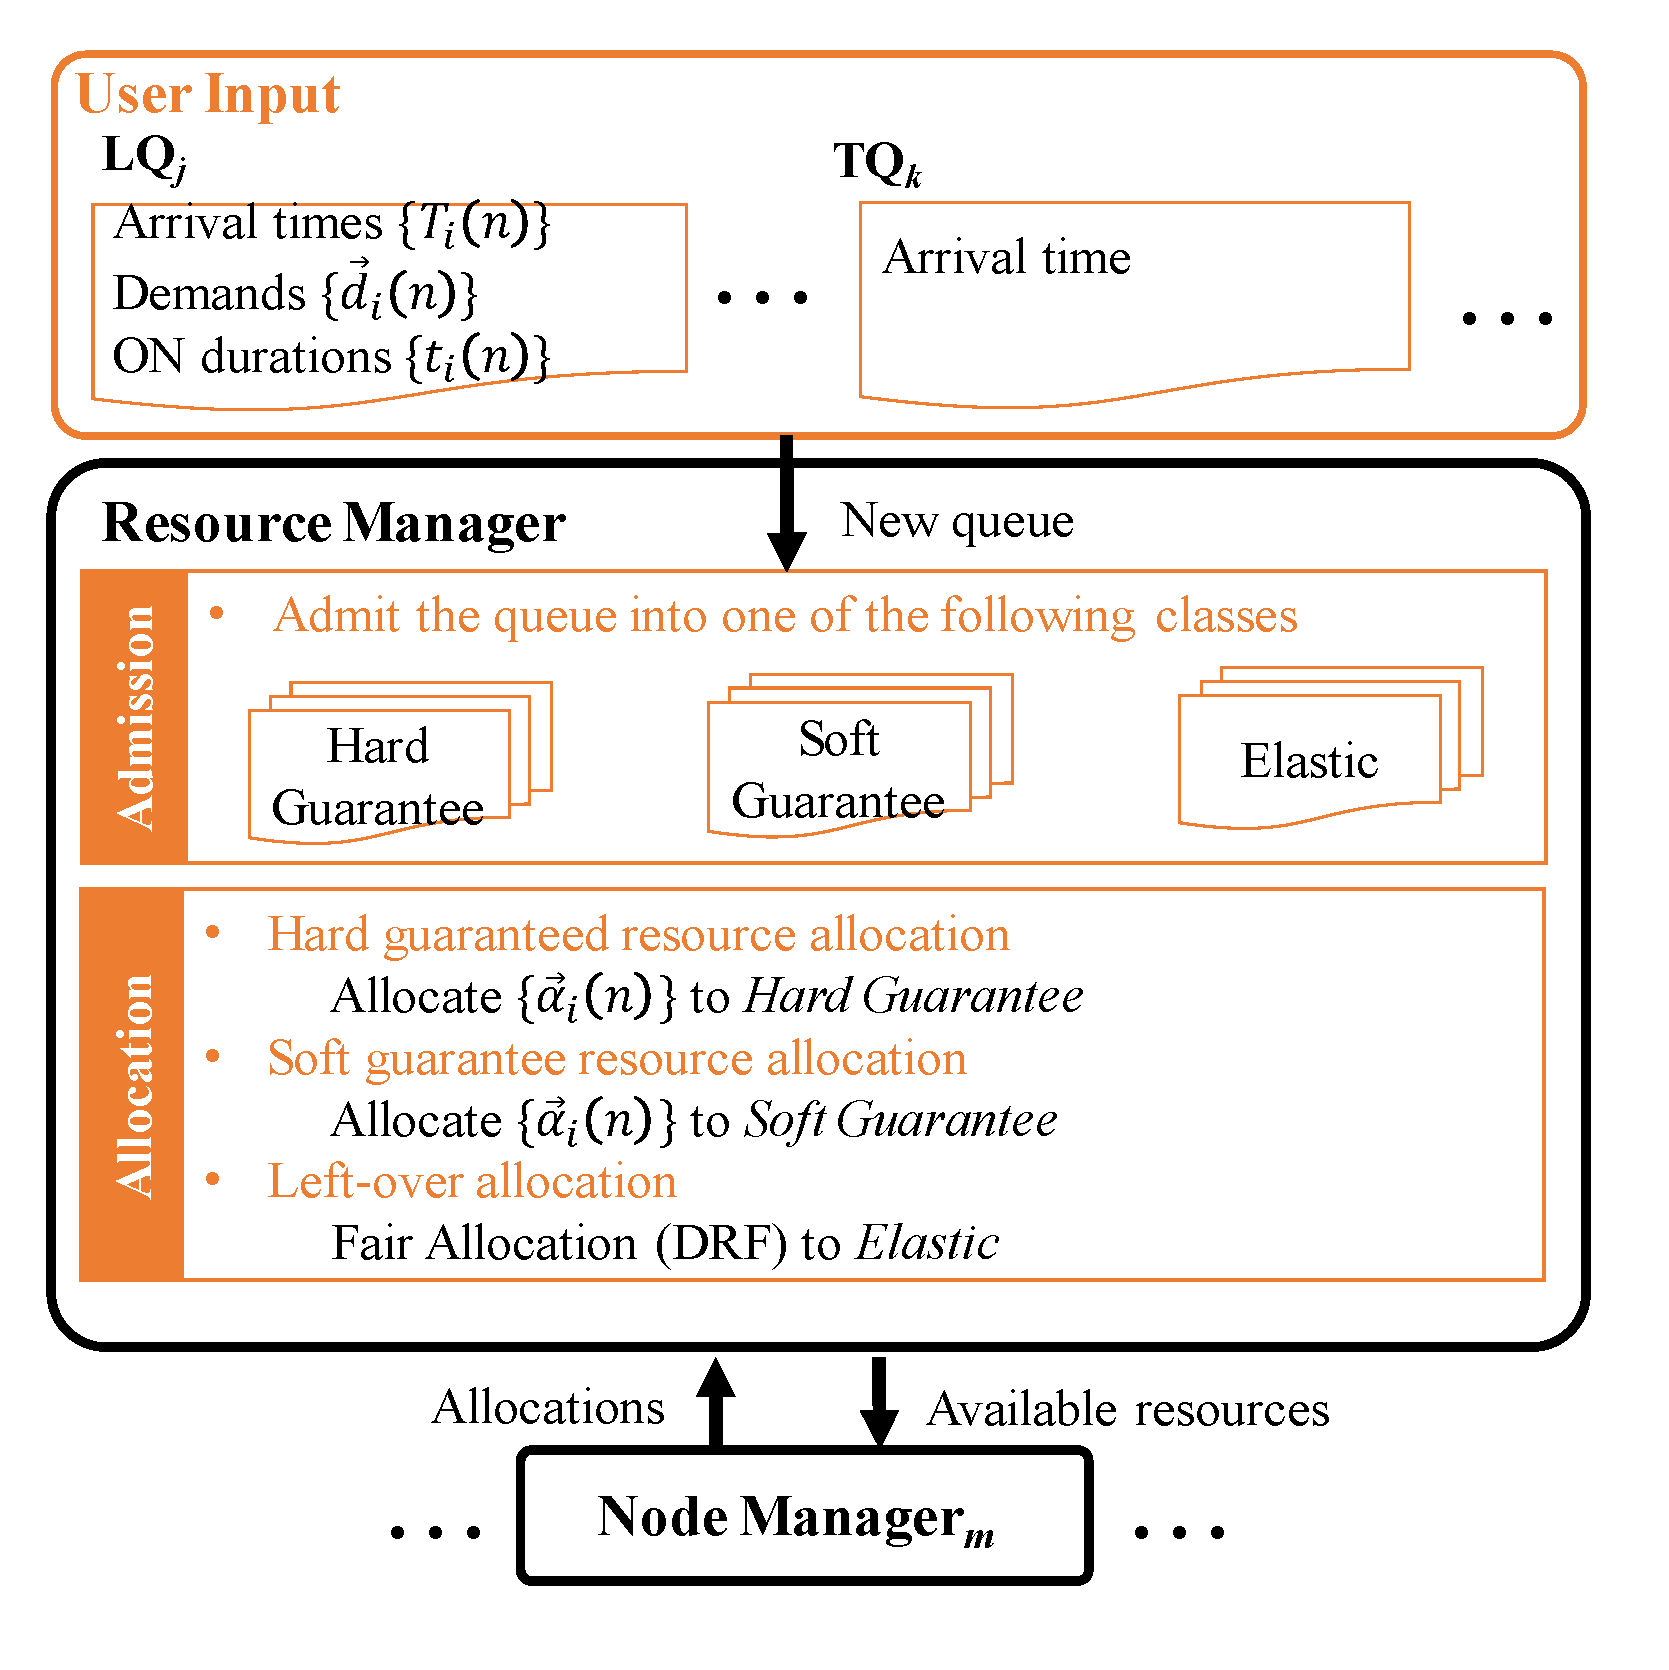
\includegraphics[width=1.0\linewidth]{fig/diagram}
\caption{Resource guarantee and long term fairness scheduling for a multiple-resource cluster. Related changes are shown in orange. \todo{User input should be changed. We should do the session admission instead of queue admission. And, users need to submit their input parameters online.}}
\label{fig:system_design}
\end{figure}

\name is implemented as a new scheduler in Apache YARN. We describe how we have implemented the three changed parts as in Figure \ref{fig:system_design}. First, our implementation requires more input from users for their job queues. Users provide their input via configuration files. More importantly, we made 2 changes in Resource Manager: admission control and \name scheduling policy. We do not touch the Node Managers.

\textbf{User Input } As LQs and TQs are treated differently, the \name scheduler requires users to provide their queues type: LQ or TQ. Recall to \ref{sec:solution_approach}, the scheduler needs some addition parameters for LQs, i.e. period, alpha, stage 1 duration, start time. Period indicates how often LQ jobs arrive. Alpha and stage 1 durations are the expected resource rate and duration to speed up LQ jobs.

\textbf{Admission } Admission for queues is not available in Yarn. The configured queues are fed into admission. If a new queue does not violate the long-term fairness, it will be admitted. Otherwise, it will be put in the best-effort queues. The \name scheduler maintains admitted LQs, admitted TQs, and the best-effort queues. 

\textbf{Allocation } We implement a new scheduling policy to achieve our goals: resource guarantee and long-term fairness. First, the scheduler maintains the resource rate for the admitted LQs. Then, the scheduler share the remaining resources to all the admitted TQs. If there is the leftover resources, they will be allocated to the best-effort queues.

\begin{table}
\centering
\caption{Important notations} 
\begin{tabular}{|c|l|} \hline
Notation & Description \\ \hline \hline
$\mathbb{A}$ & Admitted bursty queues \\ \hline
$\mathbb{B}$ & Admitted batch queues \\ \hline
$\mathbb{U}$ & Best effort (Unsatisfied) queues \\ \hline
$\myvec{R}$ & Resources \\ \hline
$\myvec{C}$ & Cluster resource capacities \\ \hline
$\myvec{L}$ & Left-over Resources \\ \hline
$\myvec{R_b}$ & Resources allocated to admitted batch queues \\ \hline
\hline\end{tabular}
\label{tbl:notations}
\end{table}

\begin{algorithm}
\caption{Scheduler}
\label{algorithm1}
\begin{algorithmic}[1]
\Procedure{periodicSchedule()}{}
\State $\{\mathbb{A}, \mathbb{B}, \mathbb{U}\}$ = \textsc{updateQueueStatus}($\mathbb{A}$,$\mathbb{B}$,$\mathbb{U}$)
\If{\textsc{isNewArrival}($\mathbb{Q}$)}
	\State Update the best effort queues: $\mathbb{U} = \mathbb{U} \cup \mathbb{Q}$
\EndIf
\State $\{\mathbb{A}, \mathbb{B}, \mathbb{U}\}$ = \textsc{admit}($\mathbb{U}$)
\State \textsc{allocate}($\mathbb{A}$,$\mathbb{B}$)
\State Obtain the available cluster resources $\myvec{L}$
\State DRF($\mathbb{U}$, $\myvec{L}$)
\EndProcedure
\\
\Function{updateQueueStatus($\mathbb{A}$,$\mathbb{B}$,$\mathbb{U}$)}{}
\ForAll{queue $A \in \mathbb{A}$}
	\If{queue $A$ is deactivated}  Update $\mathbb{A} = \mathbb{A} \setminus A$
	\EndIf
\EndFor
\ForAll{queue $B \in \mathbb{B}$}
	\If{queue $B$ is deactivated} Update $\mathbb{B} = \mathbb{B} \setminus B$
	\EndIf	
\EndFor
\ForAll{queue $U \in \mathbb{U}$}
	\If{queue $U$ is deactivated} Update $\mathbb{U} = \mathbb{U} \setminus U$
	\EndIf
\EndFor
\State \textbf{return} $\{\mathbb{A} , \mathbb{B},\mathbb{U}  \}$	
\EndFunction
\\
\Function{admit(queues $\mathbb{U}$)}{}
\ForAll{queue $U \in \mathbb{U}$}
	\If{queue $U$ is a bursty queue}
		\If{admission conditions \eqref{eqn:bursty_adm_cond_2} satisfied}
			\State Update $\mathbb{A} = \mathbb{A} \cup U$
			\State Update $\mathbb{U} = \mathbb{U} \setminus U$
		\EndIf
	\Else
		\If{admission condition \eqref{eqn:batch_adm_cond} satisfied}
			\State Update $\mathbb{B} = \mathbb{B} \cup U$
			\State Update $\mathbb{U} = \mathbb{U} \setminus U$
		\EndIf
	\EndIf
\EndFor
\State \textbf{return} $\{\mathbb{A} , \mathbb{B},\mathbb{U}  \}$	
\EndFunction
\\
\Function{\diff{allocate}($\mathbb{A}$, $\mathbb{B}$)}{}
\ForAll{bursty queue $A \in \mathbb{A}$}
		\State Compute $\myvec{a_i}$ allocated to queue $A$ as \eqref{eqn:alpha_1}, \eqref{eqn:alpha_2a}
\EndFor
\State Obtain the available cluster resources $\myvec{L}$
\State $\myvec{R_b}$ = \textsc{DRF}($\mathbb{B}$,$\myvec{L}$) as Algorithm 1 of \cite{drf}.  
\EndFunction
\end{algorithmic}
\end{algorithm}

\subsection{System Settings}

Preemption is not enabled in our Settings. Preemption is used to kill a running container of a job and create a free container for another job. Preemption has recently introduce in Fair Scheduler \cite{hadoop-fair-scheduler}. Using preemption can help the resource guarantee for LQ jobs. However, killing the tasks of running jobs may results in failure or significant delay. Hence, preemption is often disabled in practice. We do not use preemption in our system settings throughout this paper.

Container-reuse is disabled. Container-reuse has been used in some application frameworks such as Apache Tez. The objective of container-reuse is to reduce the overheads in allocating and releasing containers. The downside of container-reuse is that it cause the resource waste if the container to be reused is larger than the real demand of the new task. On the other hand, container-reuse is not possible if the new task requires more resource than the used containers. For our scheduler, we do not enable container-reuse because our scheduler periodically prefers more free resources for LQ jobs.

%In the same worker node, containers are sequentially launched. Slow allocation of containers may hurt resource guarantee.
